%% The first command in your LaTeX source must be the \documentclass command.
%%
%% Options:
%% twocolumn : Two column layout.
%% hf: enable header and footer.
\documentclass[
% twocolumn,
% hf,
]{ceurart}

%%
%% One can fix some overfulls
\sloppy

%%
%% Minted listings support 
%% Need pygment <http://pygments.org/> <http://pypi.python.org/pypi/Pygments>
\usepackage{listings}
%% auto break lines
\lstset{breaklines=true}

\usepackage{algpseudocode}
\usepackage{csquotes}

%%
%% end of the preamble, start of the body of the document source.
\begin{document}

%%
%% Rights management information.
%% CC-BY is default license.
\copyrightyear{2023}
\copyrightclause{Copyright for this paper by its authors.
  Use permitted under Creative Commons License Attribution 4.0
  International (CC BY 4.0).}

%%
%% This command is for the conference information
\conference{CLEF 2023: Conference and Labs of the Evaluation Forum, 
    September 18--21, 2023, Thessaloniki, Greece}

%%
%% The "title" command
\title{Image Retrieval for Arguments - Team "Neville Longbottom"}
\title[mode=sub]{Notebook for the Touch{\'e} Lab on Argument and Causal Retrieval at CLEF 2023}


%%
%% The "author" command and its associated commands are used to define
%% the authors and their affiliations.
\author[1]{Dascha Elagina}[%
email=daria.elagina@uni-jena.de
]
\author[1]{Bernd-Albrecht Heizmann}[%
email=bernd-albrecht.heizmann@uni-jena.de
]
\author[1]{Max Koch}[%
email=m.koch@uni-jena.de
]
\author[1]{Gustav Lahmann}[%
email=gustav.lahmann@uni-jena.de
]
\author[1]{Christian Ortlepp}[%
email=christian.ortlepp@uni-jena.de
]


\address[1]{Friedrich-Schiller University Jena,
07743, Jena}


%%
%% The abstract is a short summary of the work to be presented in the
%% article.
\begin{abstract}
  A clear and well-documented \LaTeX{} document is presented as an
  article formatted for publication by CEUR-WS in a conference
  proceedings. Based on the ``ceurart'' document class, this article
  presents and explains many of the common variations, as well as many
  of the formatting elements an author may use in the preparation of
  the documentation of their work.
\end{abstract}

%%
%% Keywords. The author(s) should pick words that accurately describe
%% the work being presented. Separate the keywords with commas.
\begin{keywords}
  CLIP \sep
  ChatGPT \sep
  IBM Debater \sep
	boilerpy
\end{keywords}

%%
%% This command processes the author and affiliation and title
%% information and builds the first part of the formatted document.
\maketitle

\section{Content extraction} \label{content-extraction}

In our approach we assume the image's stance towards a topic is reflected by the text surrounding it. Following the idea that the text in closer spacial proximity to the image in the document is more likely to be connected to the image's content, we implemented an algorithm to extract paragraphs from the document starting at the image and then alternating between paragraphs directly above and below the image. These paragraphs will be concatenated and used as the document representation for the image throughout this paper.

To find nodes containing meaningful text in the HTML document, we used the \texttt{DefaultExtractor} of the boilerpy3 library, because the default \texttt{ArticleExtractor} left out too many relevant parts of the document. The extractor employs some heuristics and marks nodes in the HTML document, which are likely to contain meaningful text, using a special tag. We then used the xPaths of the images provided in the image dataset to find image occurences in the tagged HTML document. Starting with the alt text of the image, if available, text from below and above the image is extracted alternatingly.

\begin{figure}[htbp]
	\begin{minipage}[b]{.45\textwidth}
\begin{algorithmic}
	\State $O \gets [\,]$
	\State $C \gets [\,]$
	\For{node in document}
		\If{node is tagged as content and \\ 
		\quad\quad\,\,\,node contains text}
			\State C.append(node)
		\EndIf
		\If{node.xPath in ImagexPaths}
			\State C.append(node)
			\If{O is empty}
				\State O.append(reverse(C))
			\Else
				\State O.append(C[:len(C) / 2])
				\State O.append(reverse(C[len(C) / 2:]))
			\EndIf
			\State $C \gets [\,]$
		\EndIf
	\EndFor
\State O.append(C) \\
\Return O
\end{algorithmic}
\end{minipage}
\hfill
\begin{minipage}[b]{.41\textwidth}
	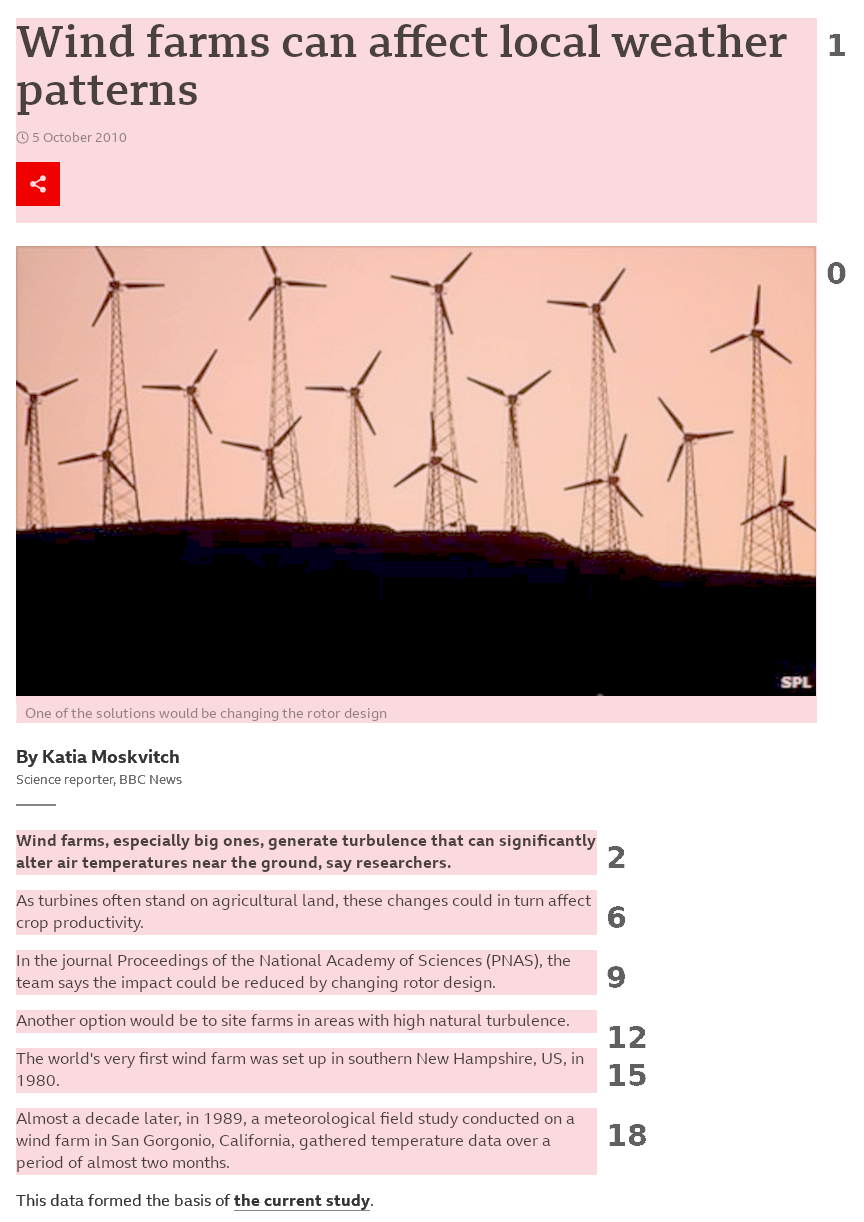
\includegraphics[width=\textwidth]{figures/bbc-news-1.png}
\end{minipage}
\vspace{.5em}
\caption{Algorithm which creates a list of lists, where the inner lists start with the image node itself followed by HTML nodes closest to the image. The text contained in the nodes in the lists will then be concatenated alternatingly starting at the front to generate a document.}
\end{figure}

\section{Query expansion}

To find arguments of a particular stance towards a given topic, we prompted ChatGPT using the following template, in which \texttt{\$STANCE} is replaced by \enquote{for} for PRO and \enquote{against} for CON. The original query is passed as \texttt{\$TOPIC}.

\begin{quote}
	Name a list of arguments \texttt{\$STANCE} "\texttt{\$TOPIC}"
\end{quote}
\begin{quote}
    For each of the arguments, what could be an image description of an image illustrating the issue?
\end{quote}

The answers were always correctly formatted Markdown lists (either enumerated or with bullet points), which could be easily parsed into a list of seperate arguments. Since our project began with the start of the public beta of ChatGPT, no official API was available yet, so the answers were fetched from the browser interface of the ChatGPT version deployed at that time using an unofficial puppeteer script. For reproducibility all answers for both stances and topics 51 to 100 are hardcoded in a text file published with our source code. \footnote{\url{https://github.com/corite/ir-code}}

\section{Retrieval}

After expanding the topic for a given stance into a list of arguments, we try to find coresponding images from the dataset in two different ways. The first one uses the surrounding text of the image, as explained in section \ref{content-extraction}, whereas the second approach exclusively works on the image data itself.

\subsection{BM25}

Using the first 4096 characters of the concatenated paragraphs obtained by the method described in section \ref{content-extraction}, a BM25 index was built for the whole dataset. The document ids are the id of the image, whose containing HTML page was used for the content extraction.

Given a list of arguments for a certain stance, we concatenate all the arguments and use the resulting string as the input query for the BM25 search, whose results will be further processed by a reranker as described later.

\subsection{CLIP}

The CLIP \cite{radford2021learning} neural network was designed and trained by OpenAI to map images as well as short phrases of text describing images into the same 512-dimensional vector space. While projects like Stable Diffusion use this model to obtain vector representaions for prompts, we wanted to find images representing a certain topic, or even argument.

For every image in the dataset we used the pretrained \texttt{openai/clip-vit-base-patch32} model to infer the corresponding vector representation, which was then normalized to length one and added to a \texttt{BallTree} index from sklearn. This enables us to use a k-nearest-neighbor search, which results in the same ranking as when sorting by cosine similarity.

Based on a list of seperate arguments, we looked up the 100 nearest images to the vector representing the argument text for each argument. The retrieval result is sorted by the distance to the respective argument, so images representing different arguments will share the top ranks. If an image appears in the 100 nearest neighbors of multiple arguments, the lowest of the distances is used as the score.

\section{Reranking}

While the retrieval operations discussed before can be efficiently applied on the whole dataset and result most of the time in on-topic images, we attempted to further refine the results towards a certain stance. For this we used the top 500 images obtained using either CLIP or BM25 and passed them to our reranking stage.

The parameters used in both rerankers were chosen using a grid search on the 2022 dataset on topics 12, 13, 20, 46 and 49, for which we manually judged the union of the top 1000 CLIP and BM25 results using the original topic as the input.

\subsection{Diff}

Often on-topic images appeared in the top results of both stances. Therefore in this reranking we subtracted 0.5 times the BM25 score of the same document for the opposite stance from the actual BM25 score, in an attempt to lower the score of neutral but on-topic images.

\subsection{Debater}

We used IBM's Project Debater Early Access API \cite{barhaim2021project} to calculate a new score for each image based on the first 5 sentences of our document representation, i.e. the sentences closest to the image in the page, including the image's alt text.

For this we used the "pro-con" endpoint, which given two sentences returns the stance of the first sentence relative to the second sentence as a number between -1 (CON) and 1 (PRO). We calculated this score for each sentence paired with the original topic text and averaged them to get the new image score. When ranking for CON instead of PRO, the score was simply inverted.

\section{Evaluation}

\begin{verbatim}
bm25_chatgpt_args.raw
bm25_chatgpt_args.diff
bm25_chatgpt_args.debater

clip_chatgpt_args.raw
clip_chatgpt_args.debater
\end{verbatim}

\bibliography{../bibliography/bibliography}

\end{document}
